\documentclass{article}

\usepackage{graphicx}

\title{Algorithmics I - Assessed Exercise\\ \vspace{4mm} 
Status and Implementation Reports}

\author{\bf Andrei-Mihai Nicolae \\ \bf 2147392n}

\date{\today}

\begin{document}
\maketitle

\section*{Status report}

Both programs are in a fully functional state. They work correctly
and, moreover, I have tried to design 2 implementations as efficient
as possible, speeding up the running time. \\
I have compiled the 2 source folders and I ran the Main classes with all the data
.txt files, as well as with a 1 million data file I created using a
bash script. They all compiled and built successfully. 

\section*{Implementation report}

\begin{itemize}
\item[(a)] 
I have implemented the Dijkstra's algorithm building up on the
skeleton pseudo-code we were given during lectures. 
\begin{itemize}
  \item Firstly, I have been careful in all classes that, when
    looping, I would in advance store the size so we won't compute it
    unnecessarily all the time. Moreover, I have chosen to use a
    visited boolean array for having quick index access while
    being inside the algorithm.
  \item Finishing with the design decisions, let's start on the actual
    algorithm implementation. We are initializing, at the beginning,
    the distances array elements with infinity, the pathList
    array (that will contain the vertex indices in the shortest path)
    elements with -1 and the visited array elements with
    false. After this, we initialize the distance to the
    sourceVertex to 0 (as we will start our search from there).
  \item Then, we go on and start the first loop that will visit all
    the nodes (however, we will stop once we get to the destination
    vertex so that we avoid unnecessary iterations).
    In there, we find out the minimum distanced vertex from 
    the last visited vertex (obviously, this minimum distanced vertex
    will be adjacent to the last visited one). 
  \item Once we've got that, we check, as mentioned above, if the
    minimum vertex found is the destination one. If so, we
    break. Otherwise, we mark it as visited and perform relaxation on
    the edges between this vertex and the adjacent nodes.
  \item Relaxation is done by updating the distances to all adjacent
    vertices if those distances could be shortened by adding the node
    to the path. If we perform relaxation, then we update
    pathList as well and add in there the minimum vertex found in the
    previous step.
  \item Last step is printing out the path. This is done recursively,
    as our nodes are in reverse order.
\end{itemize}
The time complexity of the algorithm is, at worst,
O(n\textsuperscript{2}), where n is the number of vertices in the
graph. I have obtained very good results during testing with the data
files, the ones with 2,20,40,60,80 entries giving me a running time
between 0 milliseconds and 1-2 milliseconds. The 1000 ones gave me a
running time of maximum 17 milliseconds. \\ \\
I have tested numerous approaches, including a HashSet (that does not
allow, by default, inserting duplicates), but the method I've chosen
in the end gave the best results. The biggest factors in having such a
small running time are breaking out of the loop when the destination
vertex is found, keeping track of the visited vertices using an array
of booleans, pre-computing sizes and storing them when it was
possible, as well as storing all the path vertices in an array and not
using an additional field for the Vertex class (I have tried using a
predecessor field, that would store the previously visited vertex, but
it was less efficient than the final implementation).
 
\item[(b)]
I have implemented the backtracking algorithm, again, building upon
the skeleton that was provided in the appendix of the assignment pdf. 

\begin{itemize}
\item Firstly, we will start again with design choices. I have created
  a Path class that stores a path and has the following fields:
  distance, vertices array (an arraylist of vertex indices in the path) and the
  graph associated with the Path object. The distance in my algorithm
  is automatically calculated at each insertion or removal from the path, as it
  drastically improves efficiency. Again, we use a visited array of
  booleans instead of the getVisited method for each vertex. I have
  saved the sizes/lists before each loop iteration such that we don't
  repeadetly compute the same things. 
\item The first step of the algorithm is initializing 2 Path objects,
  currentPath and bestPath. The first one will store the vertices as
  we go along and the second one will be updated once we find a
  shorter path from the source vertex to the end vertex. Moreover, we
  set the distance of the best path, when we create it, to the maximum
  possible value.
\item Then, we get the adjacency list of the last vertex in the
  current path. We loop through its nodes and, when we find an
  unvisited one, we add it to the path and mark it as visited.
\item Afterwards, we check if the current distance of the path is
  less than the best path's distance. If so, we go inside and check if
  the current vertex is the destination one or not. In the former
  case, we update the best path, while in the latter we backtrack to
  the next step.
\item In the end, we remove the last vertex in the current path and
  mark it as not visited. We print the path in the Main class looping
  through the nodes in the arraylist, as well as the distance stored
  in BestPath's field.
\end{itemize}
The running time was far greater for this algorithm. Even though for
small input the differences between Dijkstra's algorithm and this one
were not significant, for the 1000 input files the running
time was in terms of seconds, not milliseconds. For data 2,20,40,60,80
files the running time was at maximum 800-900 milliseconds, while for
the 1000 one the running time was between 17-20 seconds (on the lab
machines; on mine, it was between 12 and 14, depending on the load of
the laptop). 

\end{itemize}

\section*{Empirical results}

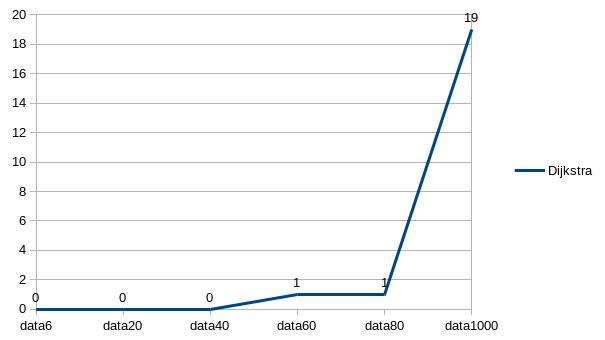
\includegraphics[width=450px,height=300px]{Dijkstra.jpg} \\
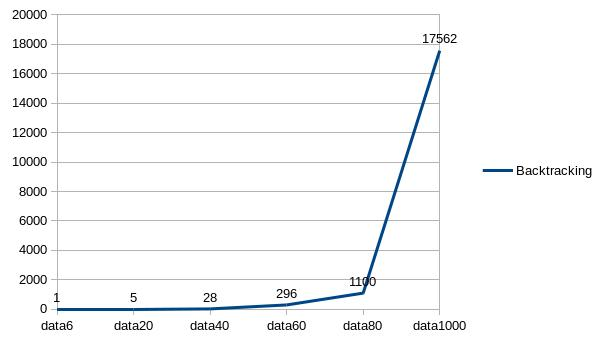
\includegraphics[width=475px,height=300px]{Backtracking.jpg} \\

These results are very conclusive right from the data ranges. The
average running time for Dijkstra's algorithm was ~4, while for
Backtracking was around ~3578 (I have included the worst running
times that I have got on the lab machines). \\ \\ 

Summing up, we have shown here that Dijkstra's algorithm is far more
efficient than Backtracking for finding the shortest path in a
adjacency list represented graph. Even though Backtracking can solve
most of the problems thrown at it, that does not mean it will also be
time/space efficient.

\end{document}
